%% ==============================
\chapter{Dimensionsreduktion}
\label{ch:Dimensionsreduktion}
%% ==============================

Die Dimensionsreduktion hat im Kern das Ziel der Abbildung eines hochdimensionalen Datensatzes auf
eine niedrigdimensionale, sogenannte \newterm{latente} Repräsentation, wobei möglichst wenig
Information über die Daten verloren gehen soll \parencite[2]{Lee.2007}. Dies ist darin begründet, dass Daten oft nur künstlich hochdimensional, also
\textit{redundant} sind. Dies bedeutet, dass die Daten effizienter über eine kleinere Menge von
Merkmalen $y_1,\ldots,y_d$ ausgedrückt werden kann, als über die ursprüngliche Repräsentation durch
die Merkmale $x_1,\ldots,x_D$ mit $d < D$ und oft $d \ll D$. Hierbei bezeichnet $D$ die
\newterm{extrinsische Dimension} des zugehörigen Ursprungsraumes $\mathcal{X}$ (welcher
üblicherweise dem $\real^D$ entspricht) und $d$ bezeichnet die \newterm{intrinsische Dimension} der
Daten. Die intrinsische Dimension wird teilweise auch als latente Dimension bezeichnet und
beschreibt die minimale Anzahl an Merkmalsvariablen $y_i$, die für die Generierung der Daten
benötigt werden \parencite[47]{Lee.2007}. Die intrinsische Dimension kann neben dieser intuitiven Sichtweise auch über
topologische Überlegungen der zugrundeliegenden Verteilung der Daten definiert werden. Diese Idee
wird in \secref{ch:Dimensionsreduktion:MannigfaltigkeitenIntrinsDim} durch das Konzept von
Mannigfaltigkeiten erläutert.

Formell wird die ursprüngliche (hochdimensionale) Repräsentation mit dem $D$-dimensionalen
Zufallsvektor $\rvect{x} = \tr{(x_1, \ldots, x_D)}$ und die latente (niedrigdimensionale)
Repräsentation mit dem $d$-dimensionalen Zufallsvektor $\rvect{y}$ gekennzeichnet. Hierbei
bezeichnet $\tr{\,(\cdot)\,}$ die Transponierte. Liegt eine konkrete Stichprobe vor, so werden die
einzelnen Stichproben $\vect{x}_i, i = 1,\ldots,n$ als Spaltenvektoren in der $n \times D$
Datenmatrix $\mat{X}$ angeordnet. Analog dazu werden die transformierten (auch: projizierten) Daten
in der Matrix $\mat{Y} \in \real^{n \times d}$ angeordnet. Es wird angenommen, dass die Datenmatrix
$\mat{X}$ \textit{zentriert} ist. Dies kann jederzeit durch Subtraktion des Erwartungswertes
$\Exp[x_i]$ einer Variable $x_i$ von Spalte $i$ sichergestellt werden.

Nachdem nun die grundlegende Terminologie und das Ziel der Dimensionsreduktion geklärt wurde,
werden im Folgenden einige weitere wichtige Ideen und Konzepte erläutert. Dazu wird in
\secref{ch:Dimensionsreduktion:FluchDerDim} der Fluch der Dimensionalität sowie in
\secref{ch:Dimensionsreduktion:MannigfaltigkeitenIntrinsDim} die Idee von Mannigfaltigkeiten und
der intrinsischen Dimension behandelt. Letztlich werden in \secref{ch:Dimensionsreduktion:Ansaetze}
kurz verschiedene Möglichkeiten der Einordnung von Dimensionsreduktionsmethoden vorgestellt.

\section{Der Fluch der Dimensionalität}
\label{ch:Dimensionsreduktion:FluchDerDim}

Sehr hochdimensionale Räume weisen einige Phänomene auf, die in niedrigdimensionalen Räumen nicht
anzutreffen sind. Diese Phänomene bereiten statistische und algorithmische Probleme und werden
unter dem Fluch der Dimensionalität (engl. \textit{Curse of Dimensionality}) zusammengefasst.
Hauptsächlich meint man damit aber die Konzentration von Normen und das Phänomen der leeren Räume.
\ldots

\section{Mannigfaltigkeiten und intrinsische Dimension}
\label{ch:Dimensionsreduktion:MannigfaltigkeitenIntrinsDim}

Wie eingangs besprochen wird bei hochdimensionalen Daten oft von Redundanz oder
Abhängigkeitsstrukturen in den Merkmalen ausgegangen. Eng damit verbunden ist die Idee, dass Daten
auf einer sogenannten \newterm{Mannigfaltigkeit} (engl. \textit{manifold}) liegen.
Dimensionsreduktionsmethoden, die auf dieser Idee basieren, gehören zu einem wichtigen Teilgebiet
der Dimensionreduktion: dem Erlernen von Mannigfaltigkeiten \parencite{Cayton.2005}. Ein Vertreter dieser Methoden ist Locally Linear Embedding, das in
\subsecref{ch:MethodenDerDimRed:statistisch:LLE} noch eingehend behandelt wird. Motiviert werden
diese Ansätze durch die Hypothese, dass reale hochdimensionale Daten in vielen Fällen auf einer in
diesem hochdimensionalen Raum \textit{eingebetteten} Mannigfaltigkeit $\mathcal{M}$ der
Dimensionalität $d$ < $D$ liegen \parencite[vgl.][1]{Cayton.2005}. In diesem Abschnitt wird ein kurzer Überblick über den abstrakten
Begriff einer Mannigfaltigkeit gegeben, wodurch ein geometrischer Bezug der intrinsischen Dimension
hergestellt werden kann.

Eine $d$-dimensionale Mannigfaltigkeit $\mathcal{M}$ ist lokal \textit{homöomorph} zum $\real^d$,
das heißt $\mathcal{M}$ ähnelt \textit{lokal} dem $\real^d$ \parencite[3]{Lee.2011}. Das bedeutet, dass es für jeden Punkt $\vect{z} \in \mathcal{M}$ eine stetige
Abbildung $\phi: B_\epsilon(\vect{z}) \rightarrow \real^d$ gibt, deren Inverse ebenfalls stetig
ist. Hierbei ist $B_\epsilon(\vect{z})$ ein Ball mit Radius $\epsilon > 0$ um $\vect{z}$. Die
Abbildung $\phi$ heißt \textit{Karte} und die Gesamtheit aller Karten ergibt den \textit{Atlas} von
$\mathcal{M}$ \parencite[4]{Cayton.2005}. Intuitiv können diese Begriffe besser anhand eines anschaulichen Beispiels
erklärt werden, weshalb in \figref{fig:Torus} ein Torus dargestellt ist. Dieses Objekt ist eine
zweidimensionale Mannigfaltigkeit eingebettet im $\real^D$.
\begin{figure}[ht]
	\centering
	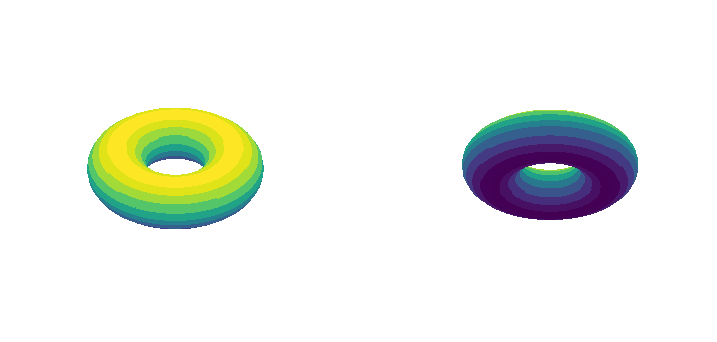
\includegraphics{torus.pdf}
	\caption[Ein Beispiel für eine zweidimensionale Mannigfaltigkeit: ein Torus]{Gezeigt ist ein Beispiel für eine zweidimensionale Mannigfaltigkeit eingebettet im $\real^3$, der sogenannte Torus. Bewegt man sich entlang der Oberfläche des Torus, so erscheint sie lokal flach und ähnelt damit dem $\real^2$. Aus diesem Grund ist der abgebildete Torus eine 2-Mannigfaltigkeit -- trotz der Tatsache, dass das Objekt als Ganzes nicht in einem zweidimensionalen Raum dargestellt werden kann. Eigene Darstellung\protect\footnotemark}
	\label{fig:Torus}
\end{figure}
\footnotetext{angelehnt an \url{https://scipython.com/book/chapter-7-matplotlib/examples/a-torus/}}
Lokal erscheint die Oberfläche des Torus flach, das heißt sie ähnelt dem $\real^2$ und nicht dem $\real^3$, in dem sie eingebettet ist. Die intrinsische Dimension im Kontext der Topologie ist also zwei. Eine Karte kann nun informell wie eine Landkarte eines Teils der Oberfläche beschrieben werden. Bewegt man sich entlang
dieser Oberfläche, so muss die Karte irgendwann gewechselt werden. Dieser Übergang von zwei sich
überlappenden Karten wird durch den Homöomorphismus $\phi$ formalisiert. Betrachtet man alle Karten
von allen Teilen der Oberfläche ergibt dies den Atlas des Torus.

Eine Mannigfaltigkeit kann darüber hinaus noch mit weiteren Eigenschaften versehen werden. Dazu
gehören glatte Mannigfaltigkeiten, auf denen Differentialrechnung möglich ist und ein sogenannter
Tangentialraum definiert werden kann. Außerdem kann zwischen zusammenhängenden und
nicht-zusammenhängenden Mannigfaltigkeiten unterschieden werden, wobei letztere aus mehreren
nicht-verbundenen Untermannigfaltigkeiten bestehen. Im restlichen Teil dieser Arbeit wird mit einer
Mannigfaltigkeit Bezug auf eine im $\real^D$ eingebettete $d$-dimensionale Mannigfaltigkeit ohne
weitere Annahmen über die Struktur (glatt, zusammenhängend) genommen. Die intrinsische Dimension
von Daten kann also auch als die topologische Dimension der im $\real^D$ eingebetteten
Mannigfaltigkeit $\mathcal{M}$, auf der die Daten liegen, definiert werden. Auf eine umfassende
formale Definition wird an dieser Stelle jedoch verzichtet. Für eine mathematisch korrekte
Definition der hier genannten Begriffe aus der Topologie wird auf \textcites{Lee.2011}{Lee.2012}
verwiesen.

\section{Einordnungen von Dimensionsreduktionsmethoden}
\label{ch:Dimensionsreduktion:Ansaetze}
Methoden der Dimensionsreduktion können auf unterschiedlichste Weise in Kategorien eingeteilt werden. Die in dieser Arbeit verwendete Kategorisierung weicht von den üblichen Kategorisierungen ab, da der Fokus hier auf dem Vergleich statistischer Methoden und Machine Learning Methoden liegt. Für einen Überblick und zur besseren Einschätzung werden in diesem Abschnitt kurz die gängigsten Kategorisierungsmöglichkeiten vorgestellt. Dazu gehört die Unterteilung in (i) lineare und nichtlineare Methoden, (ii) konvexe und nicht-konvexe Methoden, sowie (iii) Distanz- und Topologie-erhaltende Methoden.

Eine simple und weitverbreitete Unterteilung ist die in lineare und nichtlineare Methoden. Während
lineare Methoden wie die Principal Component Analysis
(\secref{ch:MethodenDerDimRed:statistisch:PCA}) nur lineare Zusammenhänge in den Daten erkennen
können, sind nichtlineare Methoden in dieser Hinsicht deutlich flexibler. Zu letzteren gehören
beispielsweise die Kernel PCA (\secref{ch:MethodenDerDimRed:statistisch:kPCA}) und die Autoencoder
(\secref{ch:MethodenDerDimRed:ML:AE}), welche eine bestimmte Klasse von neuronalen Netzen
darstellen.\rewrite{lies sich nicht gut}

\textbf{Konvexe} Methoden optimieren eine Zielfunktion, bei der jedes lokale Optimum gleichzeitig das globale Optimum ist. Die Optimierung ist daher leichter, jedoch sind die möglichen Zielfunktionen auch deutlich eingeschränkter. \textbf{Nicht-konvexe} Methoden wie der Autoencoder optimieren nicht-konvexe Zielfunktionen und können damit bei der Optimierung in suboptimalen lokalen Extrempunkten \enquote{steckenbleiben}. Die Optimierung erfolgt meist mittels des Gradientenabstiegsverfahrens (engl. \textit{gradient descent}) oder anderen mathmatischen Optimierungsverfahren \parencite[siehe z.B.][]{Guler.2010}.

\textbf{Distanz-basierte Methoden} versuchen die paarweisen Distanzen in den Daten zu erhalten, womit die zugrundeliegende Struktur erhalten werden soll \parencite[3]{Gracia.2014}. Vertreter dieser Kategorie sind die (klassische) Multidimensionale
Skalierung \parencites{Kruskal.1964}{Cox.2008}, das Sammon Mapping \addref und die Curvilinear Component Analysis
\addref. Hierbei muss eine Distanz jedoch nicht die euklidische Distanz zwischen zwei Punkten sein.
Beispielweise ist die \newterm{geodätische Distanz} als die Distanz entlang der Mannigfaltigkeit
definiert, auf der die Punkte liegen. Mit dem Hintergrundwissen zu Mannigfaltigkeiten wird jedoch
deutlich, dass euklidische Distanzen vor allem bei nichtlinearen Mannigfaltigkeiten mit einer hohen
Krümmung irreführend sein können. Die geodätische Distanz wirkt diesem Problem entgegen, ist aber
nicht immer leicht zu berechnen. Daneben gibt es \textbf{Topologie-erhaltende Methoden}, die
gezielt die Topologie der Mannigfaltigkeit erhalten wollen und dies durch geometrische Überlegungen
erzielen \parencite[4]{Gracia.2014}. Zu dieser Kategorie gehört beispielsweise das Locally Linear Embedding
(\secref{ch:MethodenDerDimRed:statistisch:LLE}), die Self-Organizing Map \parencite{Kohonen.1990} oder die Uniform Manifold Approximation and Projection (UMAP) \parencite{McInnes.2018}.

Andere Algorithmen, die in dieser Arbeit nicht vorgestellt werden können sind unter anderem Isomap \parencite{Tenenbaum.2000}, Maximum Variance Unfolding (MVU) \parencite{Weinberger.2006} und Erweiterungen von Locally Linear Embedding wie Hessian LLE \parencite{Donoho.2003} oder Local Tangent Space Alignment (LTSA) \parencite{Zhang.2002}.

Die Merkmalsextrahierung ist ein verwandtes Gebiet zur Dimensionsreduktion, da oftmals Methoden der
Dimensionsreduktion für die Merkmalsextrahierung eingesetzt werden \parencite[3]{Guyon.2006b}. Das Ziel hierbei ist es, in einem Vorverarbeitungsschritt
\enquote{irrelevante} Merkmale durch eine Transformation oder Selektion der Merkmale zu entfernen
und dann den eigentlichen Schätzer (Klassifikator oder Regressor) auf den neuen Merkmalen zu
trainieren. Insgesamt erhofft man sich durch eine Merkmalsextrahierung, dass der Klassifikator
(oder Regressor) durch robuster gegenüber Rauschen (engl. \textit{noise}) ist und eine ähnliche
oder bessere Performance bezüglich gewählter Gütemaße aufweist.\unsure{Evtl das hier ganz
	rausnehmen}

Wie wir in der Einleitung in \chapref{ch:Enleitung} gesehen haben, gibt es viele Gründe, wieso man
eine Reduktion der Dimension eines Datensatzes erreichen möchte. Unter anderem können so große
Datenmengen effizienter gespeichert werden, ohne dabei einen zu großen Informationsverlust zu
erleiden. Deswegen ist das Gebiet der Dimensionsreduktion ein immer noch aktuelles Forschungsthema
mit einer großen Bandbreite an unterschiedlichen Methoden, wie in wir in
\secref{ch:Dimensionsreduktion:Ansaetze} gesehen haben. Dem Anwender kann es mitunter schwerfallen,
den richtigen Algorithmus auszuwählen, da es laut dem dem \newterm{No Free Lunch Theorem} \parencite{Wolpert.1997} keinen \enquote{besten} Algorithmus für jede Situation gibt. Im nächsten
Schritt (\chapref{ch:MethodenDerDimRed}) werden einige dieser Algorithmen vorgestellt, die dann in
\chapref{ch:Vergleich} miteinander verglichen werden, um dem Anwender einen Anhaltspunkt für die
Auswahl einer Dimensionsreduktionsmethode zu geben.